\documentclass[../paper.tex]{subfiles}

\begin{document} Bender et al. \cite{broom-filter} introduce a different adaptive filter, called the ``broom filter''
(because it cleans up after itself). They make two key contributions to the
field of adaptive filters: describing the broom filter data structure itself,
as well as formalizing the idea of adaptivity and providing proofs regarding the guaratees
of the broom filter, and adaptive AMQs in general. The broom filter builds on
a previous AMQ called the quotient filter \cite{quotient-filter}, and, like the adaptive
cuckoo filter, consists of both a local and remote representation. In fact, one
of the main theoretical results they obtain shows that any adaptive AMQ must use
some remote (larger) storage in order to maintain adaptivity. Unfortunately, from
our experience the broom filter is quite impractical. Even a naive implementation
would be cumbersome and time-consuming to write, and important details such as
how adaptivity bits can be stored and maintained efficiently are left out.

\subsection{Quotient Filters}

The broom filter builds on a previous work called the quotient filter, which
is a non-adaptive AMQ meant to be an optimal and practical alternative to a bloom filter.
The quotient filter uses a single hash function and computes a \textit{fingerprint} for
each element inserted to the set. Given an element $x$, the fingerprint of $x$ is a
prefix of the hash $h(x)$ and is divided into two separate pieces, the \textit{quotient} with
size $q$ bits and the \textit{remainder}, with size $r$ bits. The fingerprint is therefore
the first $q+r$ bits of $h(x)$.
The quotient filter is an array of $2^q$ buckets, where
each bucket consists of $r$ bits, plus three extra metadata bits.
The sizes of the quotient and remainder are tunable
parameters of the quotient filter, which affect the false-positive probability $\epsilon$.

\textbf{Insertions and lookups:} To insert an element $x$ into the quotient filter, we first
compute the fingerprint of $x$: $p(x)$. Then we find the bucket corresponding
to the quotient and insert the remainder bits at that bucket. Assuming the bucket
is empty during insertion, a lookup for $y$ would be simple: we go to the correct bucket as given
by the quotient of $y$ and check if the remainder bits are the same. However, if the bucket is
full, linear probing is used to find an empty bucket, provided two invariants are maintained:

\begin{enumerate}
    \item All remainders with the same quotient are stored contiguously in a \textit{run}, wrapping around to the beginning if necessary.
    \item If remainder $a$ is stored before remainder $b$, then the quotient of $a$ is less than or equal to the quotient of $b$ modulo the wrapping.
\end{enumerate}

This means that inserting into a run that is followed immediately by another run may require
shifting everything in the following run over to make room.

We then have to apply the correct metadata bits to all buckets that are touched by the probe. These metadata
bits will allow us to determine which remainders correspond to which quotients,
since due to linear probing remainders will be shifted from their correct quotients.
The three metadata bits provide the following information for each bucket:

\begin{enumerate}
    \item \texttt{occupied} bit: is the bucket occupied?
    \item \texttt{shifted} bit: is the remainder stored at this bucket shifted from its corresponding quotient?
    \item \texttt{run} bit: is this bucket a part of a run?
\end{enumerate}

    Whenever a remainder is
    added, the \texttt{occupied} bit for its intended bucket is always set to 1.  If
    a remainder is not stored in its intended bucket, then the \texttt{shifted} bit
    of the bucket it is stored in is set to 1.  If the remainder has the same
    intended bucket as the remainder immediately before it, the \texttt{run} bit is set to 1.  When we
    perform a lookup for element $x$, we check the bucket indexed by the first
    $q$ bits of $h(x)$.  If \texttt{occupied} is 0, we immediately return
    \textit{absent}; otherwise, if \texttt{shifted} is 0, we scan the current run for a remainder
    that matches the remainder being looked up, and return \textit{present} if a match is found,
    and \textit{absent} otherwise.
    If the \texttt{shifted} bit is 1, then we must
    first find the beginning of the {\bf cluster}, a group of runs with no
    empty buckets between them, and then scan forward keeping track of the
    number of runs and the number of occupied buckets to determine the location
    of our target run.  If we reach the end of the cluster without finding it,
    then we return $false$, but if we do find the run, we compare to the
    remainders in that run and return $true$ or $false$ accordingly.  Deletes
    can be performed by looking up the corresponding remainder (of which their
    may be multiple) and removing it and then shifting other remainders and
    updating metadata bits as needed.

    \begin{figure}
      \centering
        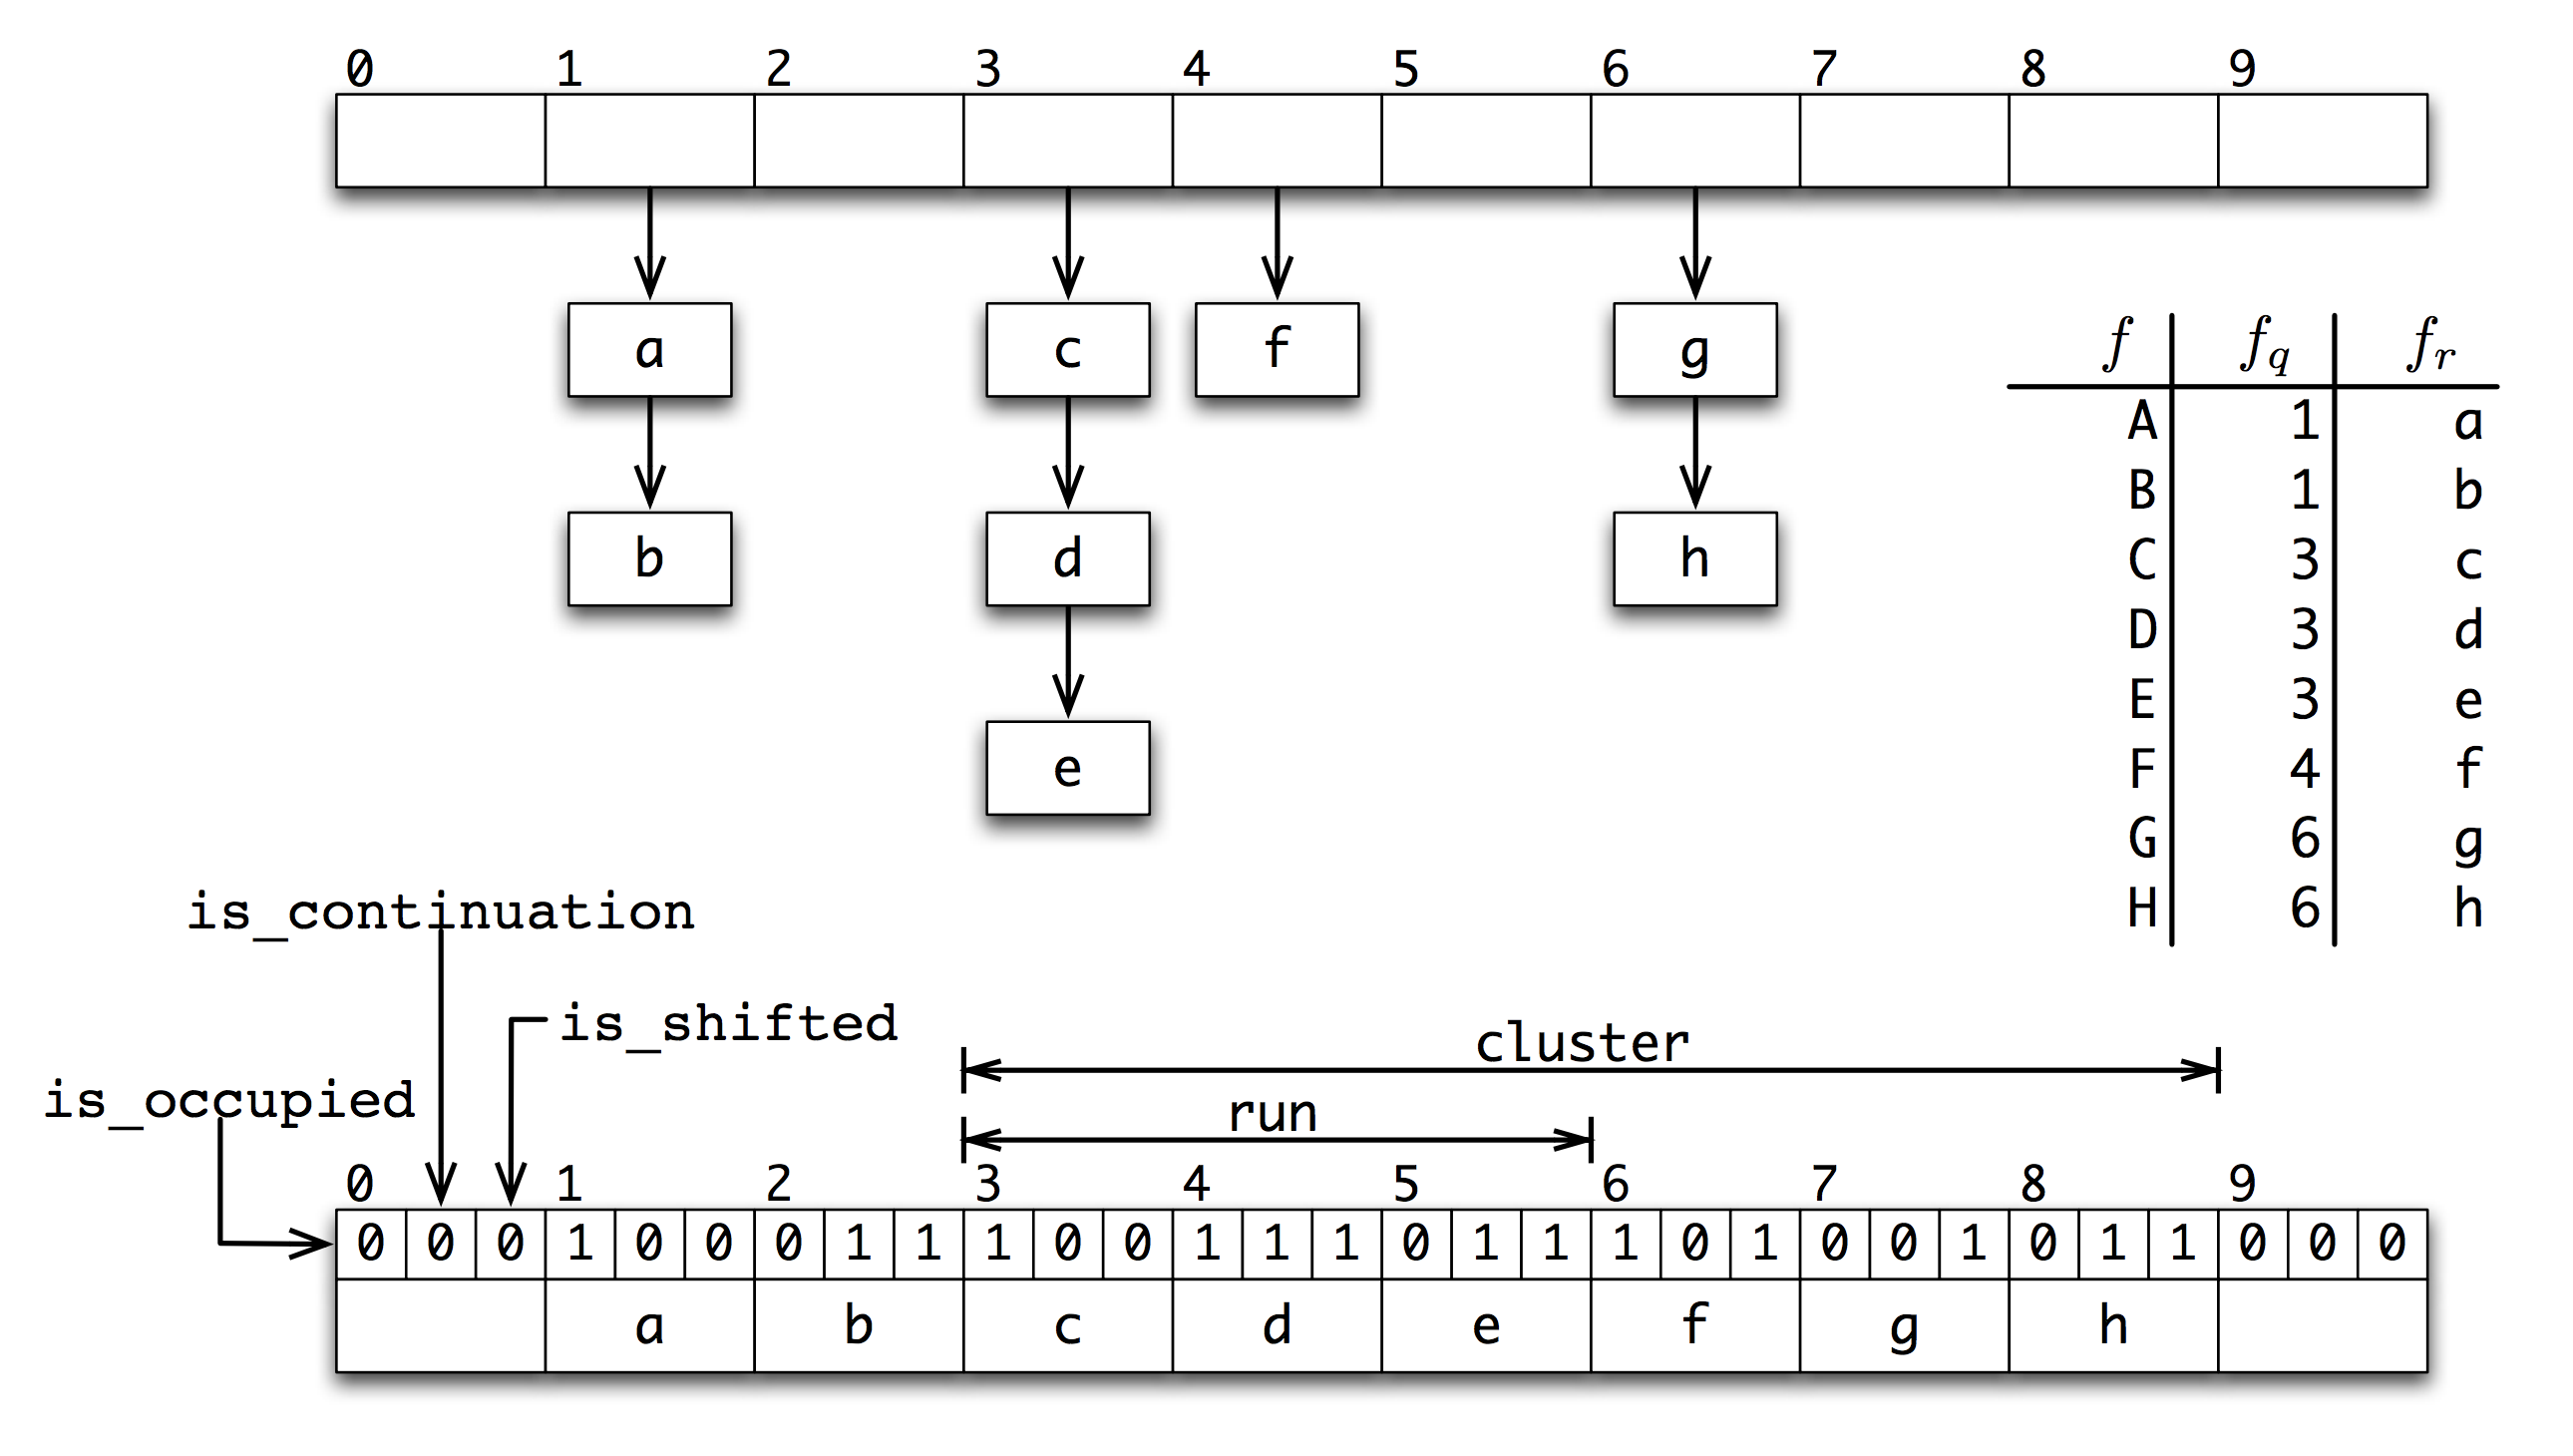
\includegraphics[scale=0.3]{qf.png}
      \label{fig:qf}
        \caption{An example quotient filter as shown in \cite{quotient-filter}. The filter has 10 slots,
        and for a fingerprint $f$, the remainder $f_r$ is stored in the bucket indexed by the quotient $f_q$. The
        remainder will be shifted from its intended bucket when there are quotient collisions.}  
    \end{figure}

% \subsubsection{Example}
    
    Let $m$ be the number of occupied buckets in the filter (the number of elements that have been inserted so far). A false positive thus occurs if $h(x) =
    h(y)$ when $x \in S$ and $y \notin S$.  Assuming $h: {\bf U} \rightarrow
    \{0, ... , 2^{q+r}-1\}$ generates outputs that are distributed uniformly
    and independently, then the probability of a false positive is given by $$
    1 - \left(1 - \frac{1}{2^{q+r}}\right)^m \approx 1- e^{-m/(q+r)} \leq
    \frac{m}{2^{(q+r)}} \leq \frac{2^q}{2^{(q+r)}} \leq 2^{-r}.$$

    If we would like to choose $r$ and $q$ such that the filter has a false-positive
    probability of at most $\epsilon$, and $n$ is the maximum set size, we can choose $q=\log(n)$
    and $r=\log(1/\epsilon)$.
    With these choices, the quotient filter achieves a false-positive probability of at most
    $2^{-r} = \epsilon$ while using $O(2^q r) = O(n \log (1/\epsilon))$ space.  	

\subsection{Adding Adaptivity}

The broom filter is a provably adaptive AMQ which makes use of quotient filters
while still providing the guarantees about the false-positive probability for
a sequence of possibly non-independent queries. The broom filter consists
of both a local and remote structure. The local partition is a fully functioning
AMQ on its own, but the remote partition is necessary to provide additional
information for adapting to false positives. Specifically, whenever there is
a false-positive caused by some element $x \notin S$, the remote structure
should provide the element $y \in S$ that caused the false-positive so
that we can modify its representation in the local AMQ so that future lookups
of $x$ will no longer result in false positives. The specific implementation
of the remote structure is not detailed, but we provide some ideas for
how it could be implemented in a later section. The need to access a remote
portion of the filter may seem counter-intuitive given that AMQs are designed
to avoid remote lookups, but the AMQ will only ever access the remote structure
when it would have been accessed anyway (to look up an item in the dictionary or
to insert an item to the dictionary).

\subsubsection{Local representation}

The details of the local representation are presented here but are tuned to
improve lookup and insert performance, rather than for enabling adaptivity,
so we only give a brief overview here.
Let $n$ be the maximum set size that will be stored by the broom filter, and $\epsilon$
be the false-positive probability of a single query.
The local representation of the broom filter consists of two quotient filters, both
with remainders of size $r=\log(1/\epsilon)$. The designs of these quotient filters
differs based on the size of the remainders. In the \textbf{small remainder} case,
where $r \leq 2 \log \log n$, both levels are quotient filters with independent hash
functions. The first layer contains $O(n)$ buckets and the second layer contains
$O(\log n/n)$ buckets. In the \textbf{large remainder} case, where $r > 2 \log \log n$,
only a single hash function is used and backyard hashing \cite{backyard-hashing} is used
to differentiate them.

Insertion and deletion in the quotient filters used by the broom filter are slightly modified to ensure constant-time
accesses. In particular, a probe limit is imposed in both cases on the first layer's quotient filter.
If a valid bucket is not found in $O((\log n)/r)$ probes (in the small remainder case) or $O(\log n / \log \log n)$
probes (in the large remainder case), then the second layer is used to execute the corresponding operation.

\begin{figure}[H]
  \centering
    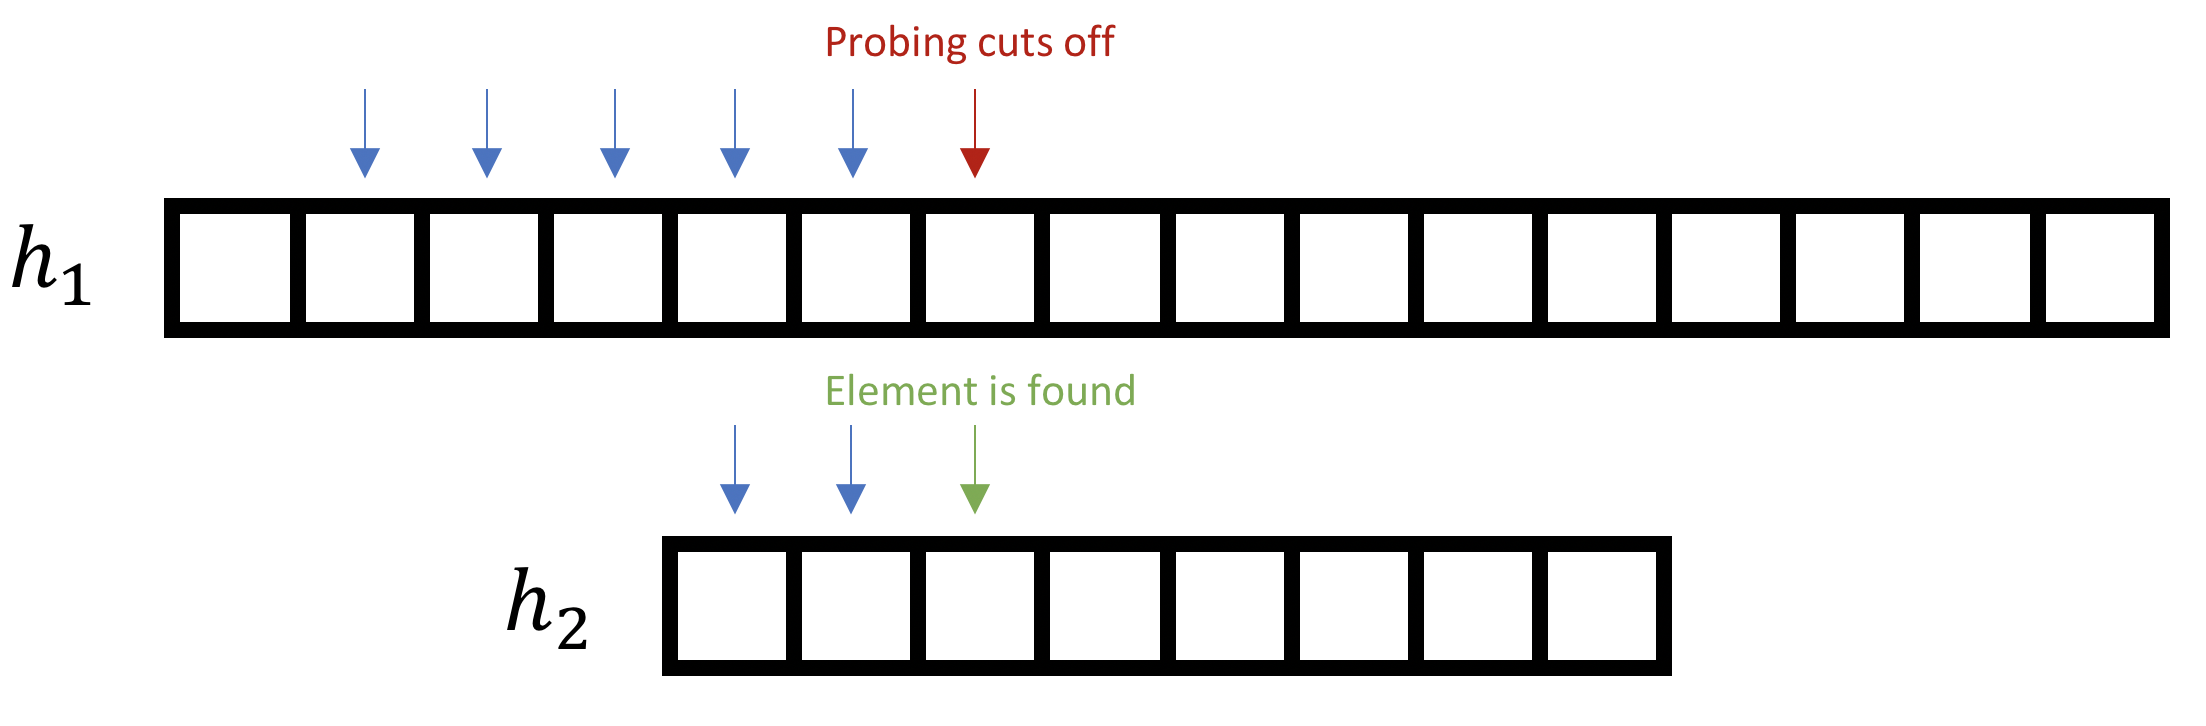
\includegraphics[scale=0.3]{probe.png}
  \label{fig:probe}
    \caption{In the small remainder case, two hash functions are used and the second layer is smaller than the first layer. Probing in the first layer is cut off after a threshold to ensure constant-time accesses.}  
\end{figure}

\subsubsection{Hash function}

The broom filter uses hash functions $h : {\bf U} \rightarrow \{0, ..., n^c\}$, for
some constant $c \geq 4$. The constant $c$ must ensure that the target set of the hash
function is large enough that the hash function is perfect and cannot cause elements
to collide. However since only a subset of the bits from the hash are used in the local
AMQ this doesn't cause space problems.

%  Suffice to say, both representations
%     require $O(n\log(1/\epsilon)$ space as well as $O(n)$ space for the
%     adaptivity bits.  

\subsubsection{Inserts, lookups, and adaptivity bits}

In the broom filter, the \textbf{fingerprint} of an element $x$ is comprised of the first
$q + r + a$ bits of the hash of $x$, where $q$ is the number of quotient bits, $r$ is the
number of remainder bits, and $a$ is the number of \textit{adaptivity} bits. The number of
adaptivity bits can vary dynamically and can be different for each element in the set. We
also maintain an invariant regarding fingerprints to make extending adaptivity bits possible.

\begin{itemize}
    \item[] \textbf{Invariant:} No fingerprint is a prefix of another fingerprint.
\end{itemize}

The adaptivity bits of a fingerprint may be extended in two cases:

\begin{enumerate}
    \item When a false-positive occurs from a lookup.
    \item When a fingerprint is added to the broom filter.
\end{enumerate}

Note that in both cases, we must access the remote structure regardless of adaptivity. A false-positive
caused by the lookup causes a lookup in the remote dictionary, and insertion requires inserting
to the remote dictionary to maintain its state correctly. Therefore in these cases we can
acquire some additional information from the remote structure for ``free'' in the sense that
the remote access is the expensive operation and must be done anyway.

To check if an item is in the set, we check if the fingerprint at each bucket is a prefix
of the item's hash, and if so, we return \textit{present}. 
If a false positive is caused by some element $x \notin S$, this means that
the fingerprint of some element $y$ in the set is a prefix of $h(x)$. If we
simply extend the fingerprint of $y$ to include more adaptivity bits until
it is no longer a prefix of $h(x)$ then $x$ will no longer cause a false positive. Extending
the fingerprint of $y$ requires accessing the full hash of $y$, which can only be
provided by the remote dictionary. Luckily, our invariant ensures that there is
only one element in the dictionary with $y$'s fingerprint, so we can find the unique
$y$.

During insertion to the broom filter, we must make sure that the invariant is maintained.
We do so by checking the newly added fingerprint against all other fingerprints with
the same quotient. If any of those fingerprints share the same remainder, adaptivity bits are
added to both fingerprints until neither is a prefix of the other (so the invariant
is maintained). Extending the fingerprints that already exist in the AMQ requires using
the same query in the remote dictionary as during the lookup described above. Note that additional
adaptivity bits may be added in this step to handle deletions as well, but this will be
explained in a later section.

It is worth mentioning that the maintenance of the
invariant and the adaptivity of the filter is dependent on the hash
function providing no collisions.  Consider if $x \notin S$, $y \in S$ and  $h(x)
= h(y)$.  In such a case, adding adaptivity bits to the fingerprint of $y$
will never make it not a prefix of $h(x)$.  This could potentially be
resolved by allowing fingerprints to grow beyond the size of their hash,
but this would likely have problematic implications for the size of the
local representation.  This does not appear to be addressed in the design
of the Broom Filter.  

\subsubsection{Deletions and cleanup}

What has been described so far is sufficient to achieve adaptivity for an AMQ that
only supports insertions and lookups, since no lookup for any given element will
ever result in a false positive more than once. However, there are two additional
features that are important to support: deletions, and space cleanup. As lookups and
insertions are performed on the broom filter, the adaptivity bits of the elements will
continue to grow, until eventually too much space is used (for example the full hash
for every item is used).
     
Deletes in the broom filter are carried out like
those in a quotient filter except that the quotient and the adaptivity
bits are not removed but are left as a {\bf ghost} in the filter.  When a
new fingerprint is added, if there is a matching ghost in the filter, then
the new fingerprint takes on all the adaptivity bits of the ghost even  if
this is more than required for the standard insert process. 
This is important because it prevents an adversary from generating false-positives
by repeatedly adding and removing an element form the filter that collides with
some element not in the filter. Since a re-inserted element retains its
adaptivity bits from before it was removed, it will not collide with any
elements that collided with it in the past.

Finally, there is the issue of continually growing adaptivity bits.
This is addressed done with a deamortized equivalent of rebuilding the the filter
every $\Theta (n)$ times adaptivity bits are extended. The broom filter keeps
two hash functions, $h_a$ and $h_b$, and has phases that
gradually switch between hash functions.  At the beginning of a phase,
frontier, we keep a counter $z = -\infty$ and only $h_a$ is used.  Once adaptivity bits are
added, the smallest constant $k > 1$ elements of $S$ that are greater than
$z$ are deleted from the filter (including their ghosts) and re-inserted
using $h_b$, after which $z$ is set to be the largest element that was
re-inserted.  This requires an access to the remote representation, but
again this will only happen when the underlying dictionary is already
being accessed (adding adaptivity bits already requires a call to the remote).
When an element is $x$ looked up or inserted, $h_a$ is
used if $x > z$ and $h_b$ is used otherwise.  Once $z$ reaches the largest
element in $S$, then a new phase begins.  This is then enough to guarantee
that, with high probability, there are $O(n)$ adaptivity bits in the
filter at any given time.  The broom filter thus achieves adaptivity while
still only using $O(n \log (1/\epsilon)$ space locally.  

\subsection{Implementation details}

Bender et al. \cite{broom-filter} provide a thorough description of the theory of
the broom filter, but some key implementation details are left out. In this section,
we provide some additional details regarding how one might implement a broom filter
and the practical issues that arise.

\subsubsection{Adaptivity bits}

Most notably, the storage of the adaptivity bits is a real problem
because they are variable-sized chunks of memory that
do not fit nicely into machine words. Storing the adaptivity
bits directly in the quotient filter for each element is a bad idea
because this means extending a fingerprint would require resizing
the entire quotient filter. Instead a better approach would be
to use a separate memory for the adaptivity bits and use some metadata
at the start to keep track of the sizes and locations of the bits for each element. Retrieving
the adaptivity bits for a certain element would require decoding the bits
from the block of memory using bitwise operations to decode across word boundaries.
Extending bits also causes the adaptivity bits array to need to be re-allocated
each time (at least this is better than re-allocating the quotient filter), and
perhaps some sort of ahead-of-time space allocation could help here too (allocating more space than
necessary so resizing isn't necessary on every extension).

In general the concept of adaptivity bits is impractical because computers perform
well when working with constant, repetitive data, which is the opposite
of what is needed to implement adaptivity bits. Small, often single-bit
extensions to variable-sized pieces of memory is an inefficient paradigm
in practice.

\subsubsection{Remote layout}

Another key detail that is not given attention by Bender et al. is the layout
of the remote data structure, and its implementation of a \texttt{RevLookup}
function, which will find the full hash of an item $x$ given by its fingerprint
$p(x)$. A naive implementation of the remote data structure would be a hashset,
and the \texttt{RevLookup} operation would need to search every item in the
set, which is very expensive. Perhaps a better solution would involve maintaining
a mapping of fingerprints to full hashes in the remote data structure. This
way, looking up the fingerprint is immediate. However this method is not easy
either, since every time a fingerprint is extended, the key in the mapping must change.
Implementing this mapping as a hash table (the obvious first thought) would prove
ineffective as extending a fingerprint would require first extending the bits of
the key and then re-hashing and re-inserting the element. Maintaining this mapping
as a radix tree seems better because extending keys is not as difficult and
we are already make sure that no key is a prefix of any other.

\begin{figure}
  \centering
    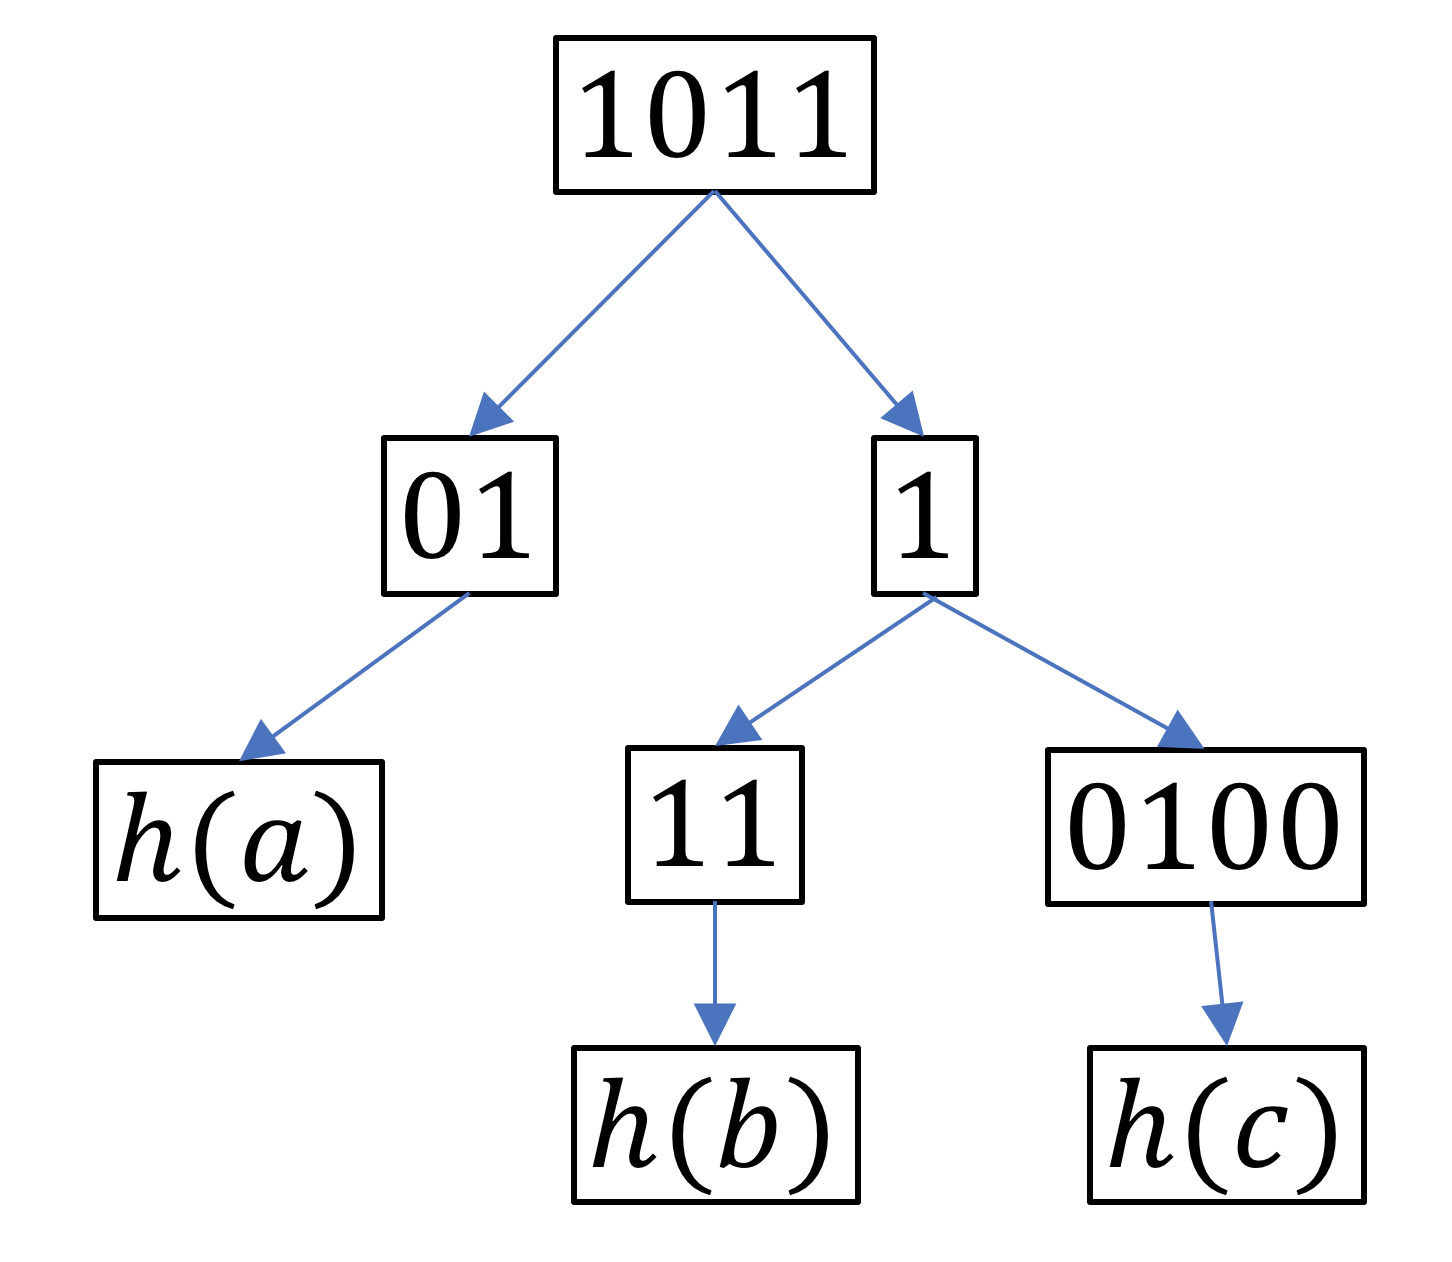
\includegraphics[scale=0.2]{radix_tree.png}
  \label{fig:radix_tree}
    \caption{Using a radix tree (compressed binary tree in this case) to map fingerprints
    to hashes. Extending adaptivity bits is much less costly with this structure than with
    a hashtable.}  
\end{figure}

\subsubsection{Hashing}

Other difficulties with implementation arise with the hash function. Bender et al.
mention that the hash function must map $U \rightarrow \{0,\ldots,n^c\}$ where
$n$ is the maximum set size and $c$ is a constant $\geq 4$. If the universe
is larger than $n^c$ then it is possible to have a complete collision between
$h(x)$ and $h(y)$. This has a low probability of occurring but if it does
occur and the colliding element is repeatedly queried, then the false positive
rate will be close to 1, causing the adaptivity of the filter to fall apart. Therefore
our hash function must hash from the universe to something larger than the universe
and be a perfect hash function to avoid these collisions. This immediately rules
out using the broom filter for strings because in that case the universe is too large.
Even with a universe of 64-bit integers (the standard case), keeping a set of size
larger than $2^{16}$ requires using a hash function that produces $>64$-bit integers.
Maintaining integers that are larger than the word size (and that may not fit in a multiple
of the word size) is often impractical and difficult.

\subsection{A Lower Bound for Adaptivity} While the
implementation of the broom filter may be impractical, the paper's theory
section offers an important insight in the design of adaptive AMQs. As part of the broom filter's design,
Bender et al. also prove that any AMQ storing a set of size $n$ from a universe
of size $u > n^4$ requires $\Omega (\min \{n\log n, n\log\log u\})$ bits of
space with high probability in order to maintain a sustained false-positive
rate $\epsilon < 1$.  This is why the remote representation is required if the
local representation is to be near the optimal size for a traditional AMQ and
why it is not surprising that the Adaptive Cuckoo Filter also shares this two
part structure.  A similar proof was explored with the {\it Bloomier Filter} 
\cite{bloomier-filter} in assessing the space required when dynamically 
updating its whitelist. The proof makes use of adversarial model where the 
goal of the adversary is to adaptively generate a sequence of $O(n)$ lookups 
that force the AMQ to either use too much space or to fail to sustain its 
false-positive rate of $\epsilon$.  
	
	{\bf The Adversary's Attack:} The adversary starts with a set $S$ of size $n$ chosen
	uniformly at random form $U$.  The attack then proceeds in rounds.  For each round, 
	a set $Q$ of size $n$ is chosen uniformly at random from $U\setminus S$.  All members
	of $Q$ are then looked up. On each subsequent round, any false-positives from the 
	previous round are queried again. 
	
	The idea of the proof is that we expect the adversary to find a certain 
	fraction of false-positives which is shown to have a high concentration using Chernoff
	bounds.  Therefore, with high probability, the AMQ will have to fix an $\epsilon$ fraction
	of false-positives in each round or fail to sustain its false-positive rate.  Each time the 
	AMQ corrects a false-positive it must change its configuration.  Each configuration of the 
	AMQ for a given set $S$ can be defined using the list of false-positives that have been
	corrected.  This results in a one-to-one mapping between the set of fixed false-positives 
	and the configurations of the AMQ.  The number of configurations can then be lower 
	bounded by the number of sets of false-positives that the adversary can force the AMQ
	to fix.  The space required for the AMQ is thus lower bounded by the amount of space 
	required to enumerate its configurations.  Finally, the bound is shown to be tight by 
	providing a construction on an AMQ, the broom filter, that uses $O(\min \{n\log n, 
	n\log\log u\})$ bits of space with high probability. 

\end{document}

